
\documentclass[12pt]{article}

% packages
\usepackage{geometry}
\usepackage{amsmath}
\usepackage{amsfonts}
\usepackage{graphicx}


\newcommand{\Q}[1]{\subsubsection*{Problem #1}}
\newcommand{\optimize}[4]
{
\begin{align*}
& \underset{#1}{\text{#4}}
& & #2 \\
& \text{subject to}
& & #3
\end{align*}
}



\newcommand{\union}[1]{\underset{#1}{\cup} }
\newcommand{\bigunion}[1]{\underset{#1}{\bigcup} \, }
\newcommand{\inter}[1]{\underset{#1}{\cap} }
\newcommand{\biginter}[1]{\underset{#1}{\bigcap} }

\newcommand{\minimize}[3]{\optimize{#1}{#2}{#3}{min}}
\newcommand{\maximize}[3]{\optimize{#1}{#2}{#3}{max}}


\newcommand{\icol}[1]{% inline column vector
  \left(\begin{smallmatrix}#1\end{smallmatrix}\right)%
}

\newcommand{\irow}[1]{% inline row vector
  \begin{smallmatrix}(#1)\end{smallmatrix}%
}
\newcommand\undermat[2]{% http://tex.stackexchange.com/a/102468/5764
  \makebox[0pt][l]{$\smash{\underbrace{\phantom{%
    \begin{matrix}#2\end{matrix}}}_{\text{$#1$}}}$}#2}

\DeclareMathOperator*{\argmax}{arg\,max}
\DeclareMathOperator*{\argmin}{arg\,min}

% parameters
\geometry{hmargin=1cm,vmargin=1cm}
\title{ORF522 - Problem Set 5}
\author{Bachir EL KHADIR }

\begin{document}



\Q{1}
\begin{enumerate}
\item Let's consider $g: u \rightarrow \log(1+e^u)$.  $g$ is
  non-decreasing and convexe because
  $g'(u) = \frac{e^u}{1+e^u} = \frac1 {1+e^{-u}}$ is increasing.

  We notice that $f(x_1, x_2) = g(x_1 - x_2) + x_2$.

  \begin{itemize}
  \item $x_2 \rightarrow x_2$ is linear
  \item $x_2 \rightarrow x_1 - x_2$ is linear, $g$ convexe and
    non-decreasing, so $g(x_1 - x_2)$ is convexe
  \end{itemize}

  c/c: $f$ is convexe.

\item
  The following transformation is a bijection from $(2, 3) \times (0, \infty) \times (0, \infty)$ to  $(\frac{\log 2}2, \frac{\log 3}2) \times \mathbb R \times \mathbb R$
  \begin{align*}
    x_1 &= 2 \log x \\
    x_2 &= \log y - \log z\\
    x_3 &= \log y
  \end{align*}

  $\frac x y  = z^2 = e^{2\log z} = e^{2 \log y - 2 x_2} = e^{2 x_3 - 2 x_2} $
  Minimizing $\frac x y$ is the same as minimizing $a(x_1, x_2, x_3) := e^{2 x_3 - 2 x_2}$
  which is convexe as the composition of a linear function
  and a convexe and increasing one $\exp$.


  \begin{itemize}
  \item
    $\frac x y = z \iff \log x - \log y = \log z \iff  \frac12 x_1 - x_3
    = x_3 - x_2 \iff \frac12
    x_1 + x_2 - 2 x_3 = 0$ and
    $b(x_1, x_2, x_3) := \frac12 x_1 + x_2 - 2 x_3$ is linear.
  \item
    $x^2 + \frac y z \le \sqrt y \iff e^{x_1} + e^{x_2}  \le \sqrt e^{x_3}
    \iff \log(e^{x_1} + e^{x_2})  \le \frac12 x_3
    \iff f(x_1, x_2) - \frac12 x_3  \le 0
    $
    and $c(x_1, x_2, x_2) := f(x_1, x_2) - \frac12 x_3$ is convexe as the sum of two convexe functions
  \end{itemize}

  c/c: the optimization problem is equivalent to:
  $$\max a(x_1, x_2, x_2) \text{ s.t. } b(x_1, x_2, x_2) = 0, c(x_1, x_2, x_2) \le 0,
  (x_1, x_2, x_2) \in (\frac{\log 2}2, \frac{\log 3}2) \times \mathbb R \times \mathbb R $$
  which is a convexe problem.
\end{enumerate}

\Q{2}

\begin{itemize}
\item[$\Rightarrow)$] Let's suppose $f$ convexe.
  \begin{align*}
    \nabla f^T(x) (y-x)
    &= \lim_{\alpha 0} \frac{f(x + \alpha(y-x)) - f(x)}{\alpha}
    \\&= \lim_{\alpha 0} \frac{f((1-\alpha)x + \alpha y) - f(x)}{\alpha}
    \\&\le \lim_{\alpha 0} \frac{(1-\alpha)f(x) + \alpha f(y) - f(x)}{\alpha} &\text{(because $f$ convexe)}
    \\&\le f(x) - f(y)
  \end{align*}
\item[$\Leftarrow)$] Let's suppose $\forall x, y \, \nabla f^T (y-x) \le f(y) - f(x)$
  
  Let $\alpha \in (0, 1)$, and $u = (1-\alpha)x + \alpha y$
  
  $$f(x) - f(u) \ge \nabla f(u) (x-u)$$
  $$f(y) - f(u) \ge \nabla f(u) (y-u)$$

  By multiplying the first ineqaulity by $1-\alpha$ and the second one by $\alpha$ and summing, we get:
  $(1-\alpha) f(x) + \alpha f(y) - f(u) \ge 0$

  Which proves that $f$ convexe.
\end{itemize}


\Q{3}
\begin{enumerate}
\item
  $D$ being definite positive, It can be written as a diagonal matrix in an orthonormal basis.
  Since  rotations are isometries, witout loss of generality we can assume that $D = \operatorname{diag}(d_1, ... d_n) $ is diagonal in the canonical basis.
  Let's call $\lambda$ the biggest of the eigen values of $D$, and $\beta$ the smallest.

  let's define the norm $||u||_D^2 := u^T D^{-1} u = ||\sqrt{D^{-1}}u||_2^2$ and the associated scalar product $<.,.>_D$
  We have that: $ \frac{||u||_2^2}{\lambda} \le ||u||_D^2 \le \frac{||u||_2^2}{\beta}$
  
  We assume that the projection $[.]^+$ is done with
  respect to the norm $||\, ||_D$ rather than the euclidian norm.
  Let $y_{k+1} := x_k - \alpha D \nabla f(x_k)$ such that $x_k = [y_k]^+$

  \begin{align*}
    f(x_k) - f(x^*) & \le \nabla f(x_k) (x_k - x^*) \\
                    &= \frac1 \alpha (D^{-1}(x_k - y_{k+1}))^T (x_k - x^*) \\
                    &= \frac1 {2\alpha} ( ||x_k - y_{k+1}||_D^2 + ||x_k - x^*||_D^2 - ||y_{k+1} - x^*||_D^2 ) \\
  \end{align*}
  Since $\nabla^2f$ is uniformly bounded by $||H||$, we have that $\nabla f$ is $L$-Lipschiz.
  We assume that $$\nabla f$$ is uniformly bounded by a constant $L$.

  And By non expansiveness of the projection $[.]^+$:  $||y_{k+1} - x^*||_D \ge ||x_{k+1} - x^*||$
  So:
  $$f(x_k) - f(x^*) \le \frac 1{2\alpha} (\alpha^2 L + ||x_k - x^*||_D^2 - ||x_{k+1} - x^*||_D^2)$$
  By summing over $k$:
  $$\sum_{i \le k} (f(x_i) - f(x^*)) \le \frac{k}2 \alpha L + \frac{1}{2\alpha} ||x_0 - x^*||_D^2$$

  Let's show that $f(x_i)$ is non-increasing. Indeed, We have that
  \begin{itemize}
  \item
    By non expansiveness of the projection:
    $$\nabla f(x_k) (x_{k+1} - x_k) = -\frac 1{\alpha}
    (y_{k+1}-x_k)'D^{-1}(x_{k+1} - x_k) =-\frac1 {\alpha}
    <y_{k+1}-x_k, x_{k+1} - x_k>_D \le -\frac1{\alpha}
    ||x_{k+1}-x_k||_D^2$$
  \item
    By Cauchy Schwartz and the non expansiveness of the projection:
    \begin{align*}
      ||x_{k+1}-x_k||_2^2 &\le \lambda ||x_{k+1}-x_k||_D^2 \\
                          &\le \lambda ||y_{k+1}-x_k||_D^2 \\
                          &\le \alpha^2 \lambda  \nabla f(x_k)'D \nabla f(x_k) \\
                          &\le \alpha^2 \lambda^2 ||\nabla f(x_k)||_2^2 = \alpha^2 \lambda^2 L^2
    \end{align*}
  \item
    Taylor approximation:
    \begin{align*}
    f(x_{k+1}) - f(x_k) &\le \nabla f(x_k) (x_{k+1} - x_k) + \frac12 ||H||^2 ||x_{k+1} - x_k||_2^2 \\
                        &\le -\frac1 {\alpha}   ||x_{k+1} - x_k||_D^2 + \alpha^2 \frac{\lambda^2 L^2 ||H||^2}2 
    \end{align*}
    Which is smaller than $0$ when $\alpha$ is small enough.
    Therefore:
    $f(x_k) - f(x^*) \le \frac1k \sum_{i \le k} (f(x_i) - f(x^*)) \le \frac{\alpha L}{2} + \frac{1}{2\alpha k} ||x_0 - x^*||_D^2$

  \end{itemize}
  
  
As a result:
$$f(x_k) - f(x^*) = \min_{i \le k} f(x_i) - f(x^*) \le \frac1k \sum_{i \le k} (f(x_i) - f(x^*)) \le \frac{\alpha L} {2}  + \frac{||x_0 - x^*||_D^2}{2\alpha k}$$

\item

  Let $g: \alpha \rightarrow \frac{\alpha L} {2}  + \frac{||x_0 - x^*||_D^2}{2\alpha k} := a \alpha + \frac{b}{\alpha}$ so that
  $g'(\alpha) = a - \frac{b}{\alpha^2}$, $g''(\alpha) = \frac{2b}{\alpha^3} > 0$

  $g$ is convexe, so it is minimal when $g'(\alpha) = 0$, ie
  
  $\alpha = \sqrt{\frac b a} = \sqrt{\frac{||x_0-x^*||_D^2}{Lk}}$,
  $\min g = g(\alpha) = 2 \sqrt{\frac{b}{a}} = 2\sqrt{\frac{||x_0-x^*||_D^2}{Lk}}$

  Therefore the optimal bound is:
  $$f(x_k) - f(x^*) \le \sqrt{\frac{||x_0-x^*||_D^2}{Lk}} = O(k^{-\frac12})$$

\item 
  Since $\nabla f$ is Lipshiz:  $||\nabla f(x_k) - \nabla f(x^*)||_2 \le ||H|| ||x_k - x^*||_2^2$
  We will also need the inequality: $||Du||_D \le \frac{||Du||_2}{\beta} \le \frac{\lambda}{\beta} ||u||_2$
  And the fact that $x^* = [x^* - \alpha D \nabla f(x^*)]^+$
  
  \begin{align*}
    ||x^{k+1} - x^*||_D^2 & \le || [x_k - \alpha D \nabla f(x_k)]^+ - [x^* - \alpha D \nabla f(x^*)]^+||_D^2 \\
                          & \le || x_k - x^* - \alpha D(\nabla f(x_k) - \nabla f(x^*))||_D^2 \\
                          & \le ||x_k - x^*||_D^2 - 2 \alpha <D(\nabla f(x_k) - \nabla f(x^*)), (x_k - x^*)>_D + \alpha^2 ||D (\nabla f(x_k) - \nabla f(x^*))||_D^2 \\
                          & \le ||x_k - x^*||_D^2 - 2 \alpha (\nabla f(x_k) - \nabla f(x^*))' (x_k - x^*) + \alpha^2 \lambda^2 ||\nabla f(x_k) - \nabla f(x^*)||_2^2 \\
                          & \le ||x_k - x^*||_D^2 - 2 \alpha \sigma ||x_k - x^*||_2^2+ \alpha^2 \frac{\lambda^2}{\beta^2} ||H|| ||x_k - x^*||_2^2 & \text{By strong convexity}
    \\                    & \le ||x_k - x^*||_D^2 - 2 \alpha \frac{\sigma}{\beta^2} ||x_k - x^*||_D^2+ \alpha^2 \frac{\lambda^2}{\beta^4} ||H|| ||x_k - x^*||_D^2 & \text{By strong convexity}
    \\                    & \le (1 - 2\frac{\sigma}{\beta^2} \alpha + \frac{||H|| \lambda^2}{\beta^4} \alpha^2)||x_k - x^*||_D^2
    \\ & \le \rho ||x_k - x^*||_D^2 \\& (\rho = 1 - 2\frac{\sigma}{\beta^2} \alpha + \frac{||H|| \lambda^2}{\beta^4} \alpha^2)
    \\ & \le \rho^{k+1} ||x_0 - x^*||_D^2 \\&\text{By reccurence}
  \end{align*}

\item
  $\rho$ is quadratic in $\alpha$, so it is minimal when $\frac{\partial \rho}{\partial \alpha} = 0 $, ie $\alpha = \frac{\beta^2\sigma}{||H|| \lambda^2}$,
  $\min \rho = 1 - \frac{\sigma^2}{||H|| \lambda^2}$
\end{enumerate}

 
\Q{4}
\begin{enumerate}
\item
  For $y \in \mathbb R^n$
  $\sup_y L(x, y) \ge L(x, u)$

  By taking the $\inf_x$:
  $\inf_x \sup_y L(x, y) \ge \inf_x L(x, u)$

  By taking the $\sup_u$:
  $\inf_x \sup_y L(x, y) \ge \sup_u \inf_x L(x, u)$

\item

  Let $f(x) := \max_y L(x, y)$
  We know that $x^* \in \argmin f$ and $f$ is convexe,
  so $\partial f(x^*) = 0$.

  $L$ is continuous the Danskin's theorem, we have that:
  $0 \in \{ \nabla_x L (x^*, y) | y \in \argmin L(x^*, y^*) \} = \{ \nabla_x L (x^*, y^*) \}$ , wich means that
  $\nabla_x L (x^*, y^*) = 0$, and symmetrically, $\nabla_y L (x^*, y^*) = 0$.

  c/c:
  \begin{align*}
    x^* &= x^* - \alpha \nabla_x L (x^*, y^*)\\
    y^* &= y^* - \alpha \nabla_y L (x^*, y^*)
  \end{align*}
  
\end{enumerate}

\Q{5}
\begin{enumerate}
\item Let's call $S_t$ the price of the stock at time t, and $V_t(S_t)$ the
  price of the corresponding american action (with strike $K$)
  \begin{itemize}
  \item State $x_t = S_t$, $t = 1..T$
  \item Action:
    \[
      u_t = \left\{ \begin{array}{cc}
                      \text{EXEC} & \text{meaning we exercise the option}\\
                      \text{HOLD} & \text{meaning we don't}
                    \end{array}
                  \right.
                \]
              \item Randomness: The change in the stock price
                $w_t = \frac{S_{t+1}}{S_t}$ s.t $x_{t+1} = w_t x_t$, $P(w_t = u) = 1 - P(w_t = d) = p$
              \item Transitional cost:
  
                $g(x_k, u_k=\text{HOLD}, w_t) = 0$
                $g(x_k, u_k=\text{EXEC}, w_t) = x_t-K$
                $g(x_T) = (x_T - K)^+$: We exericse the option at time $T$ only if $x_T > K$
              \end{itemize}
              The price problem:
  $$V_k(x) = \max_{\mu} E[g(x_T) + \sum_{t=k}^{T-1} g(x_k, \mu_k(x_k), w_t) | x_k = x]$$

\item Bellman equation:
  $$V_k(x) = \max \left\{ x-K , p V_{k+1}(u x) + (1-p) V_{k+1}(d x) \right\}$$
  $$V_T(x) = (x-K)^+$$
  Result for $K = S_0 = 1., P(w_t = \text{down}) = 0.45, \text{up} = 1.1, \text{down} = 0.9, T = 100 \text{ days}, \text{time step} = 10$:
 
  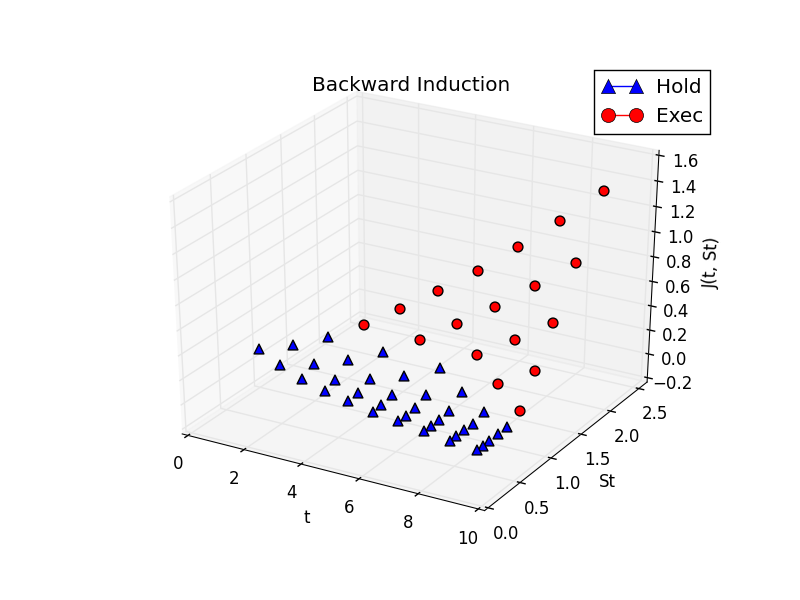
\includegraphics[scale=1.]{qtree.png}

\item
  
  LP:
  Let $J(t, S)$ be the price of the option at time $t$ is $S_t = S$,
  and we decide to adopt the strategy 

  $J$ verifies: $J(t, S) = \max \{ E[J(t+1, S_{t+1}) | S_t = S], S - K \} = [\max_{\mu} (P_{\mu}J + g_\mu) ](t,S) $
  where:
  $$\mu(t, S) \in \{ \text{HOLD}, \text{EXEC} \}$$
  \[ (P_\mu J)(t, S) = \left\{
      \begin{array}{cc}
        p J(t+1, uS) + (1-p)J(t+1, dS) & \text{ if $\mu(t, S) = $ HOLD } \\
        0 & \text{otherwise}
      \end{array}
    \right.
  \]
  \[
    g_\mu(t, S) = \left\{
      \begin{array}{cc}
        0 & \text{ if $\mu(t, S) = $ HOLD } \\
        S - K & \text{otherwise}
      \end{array}
    \right.
  \]

  The LP problem is:
  $$\min e^T J \text{ s.t } \forall \mu \, J \ge P_\mu J + g_\mu$$
  At time $t$, $S$ can take the following values $\{ u^k d^{t-k} S_0,\, k \le t\}$. Let's denote by $\tilde J(t, k) := J(t, u^k d^{t-k} S_0)$ when $k \le t$ and $L$ otherewise where $L >> S_0$ is a very big constant.
  The problem can be written as:
  \begin{align*}
    \min &\sum_{t, k} \tilde J(t, k) \\
         &\text{ s.t } \forall t, k \in \{1...T-1\}\\
         & \tilde J(t, k) \ge p \tilde J(t+1, k) + (1-p) \tilde J(t+1, k+1) \\
         & \tilde J(t, k) \ge u^k d^{t-k} S_0 - K\\
         & \tilde J(T, k) = u^k d^{t-k} S_0 - K \\
         & \tilde J(t, k) = L \text{ when } k > t\\
  \end{align*}

  Let $x_{t*T + k} = \tilde J(t, k)$, and define $A \in \mathcal M_{T^2, T^2}$,
  $B \in \mathcal M_{\frac{T(T-1)}{2}, T^2}$ $U \in \mathbb R^{T^2}$ such that:

  \[
    A := 
    \begin{array}{r@{}}
      \text{T(T-1)}~\left\{\begin{array}{@{}c@{}}\null\\\null\\\null\end{array}\right.\\
      \text{T}~\left\{\begin{array}{@{}c@{}}\null\\\null\end{array}\right.\\
    \end{array}
  \left [
    \begin{array}{ccccc}
      0               & p                     & (1-p)  & 0     & \cdots \\
      \vdots          &                       & \ddots & \ddots& \cdots \\
      0               &                       & \cdots & p     & (1-p)  \\
      0               & 0                     & 0      & 0     & 0      \\
                      & \cdots                & \cdots &       & 
    \end{array}
  \right ]
\]


  \[
    B := 
    \begin{array}{r@{}}
      \text{T-1}~\left\{\begin{array}{@{}c@{}}\null\\\null\\\null\end{array}\right.\\
      \text{T-2}~\left\{\begin{array}{@{}c@{}}\null\\\null\\\null\\\null\end{array}\right.\\
      \text{\vdots}~\left\{\begin{array}{@{}c@{}}\null\end{array}\right.\\
      \text{T - (T-1)}~\left\{\begin{array}{@{}c@{}}\null\end{array}\right.\\
    \end{array}
  \left [
    \begin{array}{cccc|ccccc|c|ccc}
      0 & 1      &        &\cdots &&& &&& &&& \\
        &        & \ddots &       &&& &&& &&& \\
        &        &        & 1     &&& &&& &&& \\
      \hline
        &        &        &       & 0 & 0 & 1 & \cdots &   &&&&\\
        &        &        &       &   &   &   & \ddots &   &&&& \\
        &        &        &       &   &   &   &        & 1 &&&&\\
      \hline
        &        &        &       &   &   &   &        & & \ddots \\
      \hline
        &        &        &       &   &   &   &        & &        & 0 & \cdots & 1 \\
    \end{array}
  \right ]
\]
 $U \in R^{T^2}$ such that : $U_{tT + k} := u^kd^{t-k}S_0 - K$

 The LP problem is equivalent to:
 \begin{align*}
    \min & e^T x \\
         &\text{ s.t } \\
         & x \ge Ax \\
         & x \ge U\\
         & Bx = L 1_{\frac{T(T-1)}2}
  \end{align*}
 
  Result for the same parameters as before:
  
  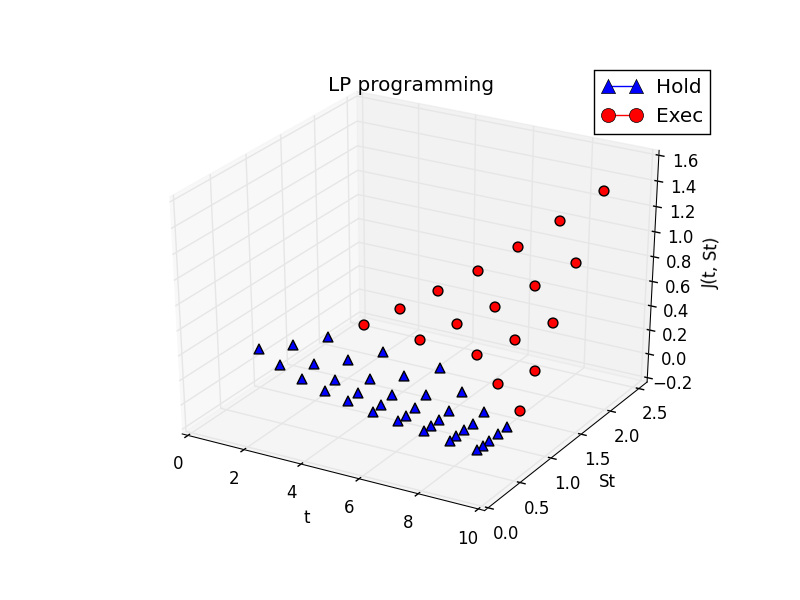
\includegraphics[scale=1.]{qlp.png}  
\end{enumerate}

\Q{6}

\begin{itemize}
\item
  We choose a discrete random walk model for generating $S_t$:
  $S_t = Y + \sum_{i \le t} X_i$ where
  the $X_i$ are iid $\mathcal{N}(\mu, sigma)$
  and $Y$ uniform on $\{-10, ..., 10\}$ and independent from the $X_i$

  Sample trajectories:
  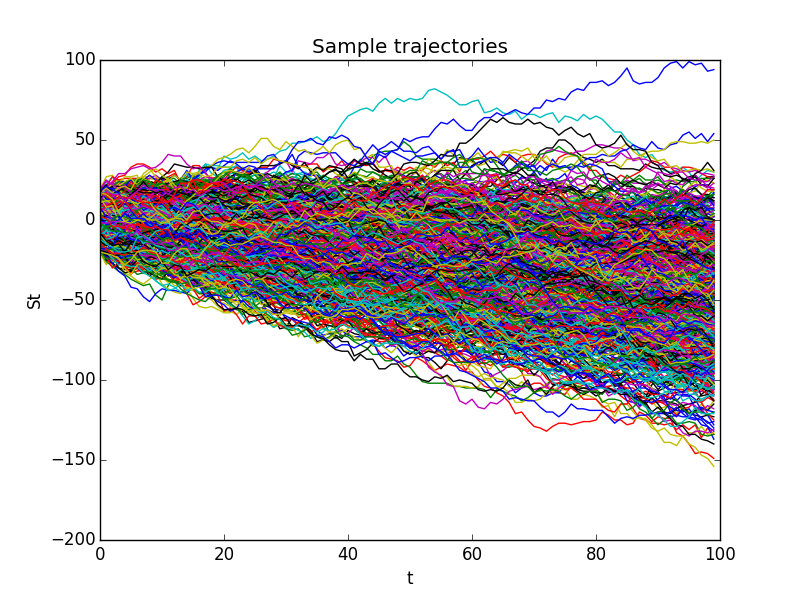
\includegraphics[scale=1.]{traj.png}
  
\item 
  By generating the paths $(S_t^{(i)})_i$,
  we simulate the transitions $(t, S_t) \rightarrow (t+1, S_{t+1})$

    We adopt the same notation as in lecture 23 slide 36.
    At step $i \in \{0, ..., M-1\}$:
    $$Q_{i+1}((t, S_t)) =  (1-\gamma)Q_i((t, S_t)) + \gamma \max( S_{t+1} - K, Q_i((t+1, S_{t+1}))$$
    
    $$J((t, S_t)) = \max \{ S_t - K, Q_M((t, S_t)) \}$$

    
    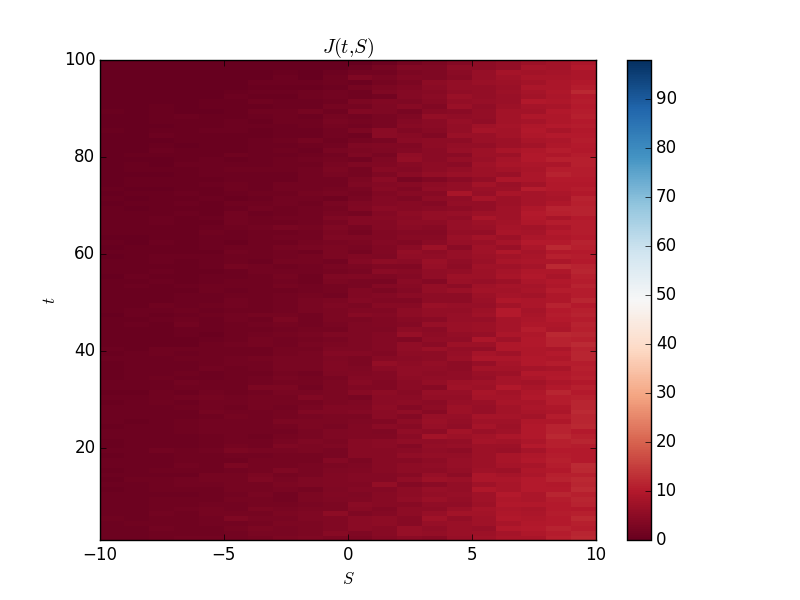
\includegraphics[scale=1.]{option.png}
    
    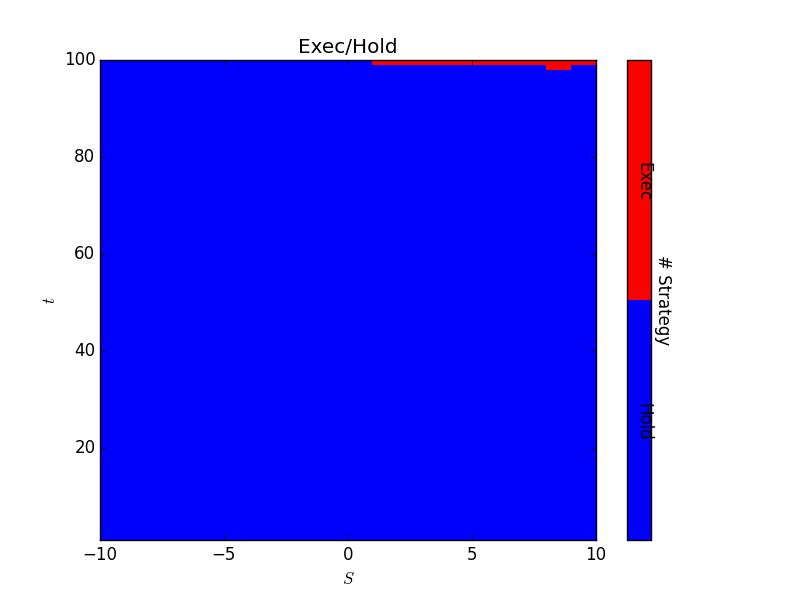
\includegraphics[scale=1.]{control.png}
\end{itemize}
\end{document}

%%% Local Variables:
%%% mode: latex
%%% TeX-master: t
%%% End:

























